\documentclass[11pt]{article}
\usepackage[margin=2.5cm]{geometry}
\usepackage[T1]{fontenc}
\usepackage{lmodern}
\usepackage{graphicx}
\usepackage{booktabs}
\usepackage{amsmath}
\usepackage[numbers,sort&compress]{natbib}
\usepackage[hidelinks]{hyperref}
\usepackage{setspace}
\onehalfspacing

\title{Adjustment and external replication of drug--hearing-loss signals in FAERS:
a disproportionality analysis of FAERS and Canada Vigilance}
\author{Oleg Tropynin\\ \small Independent researcher, Karaganda, Kazakhstan\\ \small \texttt{tropininoleg@gmail.com}}
\date{}

\begin{document}
\maketitle

\begin{abstract}
\noindent\textbf{Introduction:} Recent disproportionality analyses of the FDA Adverse Event Reporting System (FAERS)
reported many drug--hearing-loss signals absent from labels. We assessed which survive adjustment for hearing-specific biases
and external replication.

\noindent\textbf{Methods:} Disproportionality analysis of 19.9 million deduplicated FAERS reports
(2004--2026) and 1.2 million Canada Vigilance reports, following a protocol committed before
analysis. For hearing loss and tinnitus, crude reporting odds ratios (ROR; signal: lower 95\% bound $>1$, $\geq$3 cases) were
compared with Mantel--Haenszel estimates stratified by age, sex and period after excluding ear-related indications, reports
naming established ototoxic drugs and lawyer reports. Methods were compared on a label-derived reference set (area under the
ROC curve, AUC) and by replication in Canada Vigilance, observed and power-calibrated; robust unlabelled signals underwent
case-by-case review.

\noindent\textbf{Results:} Adjustment changed the hearing-loss signal list (300 crude, 310
adjusted, 63 lost) but not agreement with labels (AUC 0.718 vs
0.723). Labelled signals replicated in Canada as often as predicted (observed/expected
1.00); unlabelled signals did not (0.42;
post hoc, both databases adjusted: 0.20). Solicited patient-support-programme
reports and shared co-medication produced spurious replications. Of 22 robust unlabelled hearing-loss and tinnitus signals
(post hoc), 18 were attributed to report clusters, stimulated reporting, indication or an established class;
4 remained, led by pregabalin.

\noindent\textbf{Conclusions:} Most unlabelled FAERS hearing-loss signals do not survive adjustment, adjusted replication and
provenance review. These findings are hypothesis-generating; cross-database replication needs adjusted estimates and explicit
handling of solicited reports.
\end{abstract}

\section*{Key points}
\begin{itemize}
\item Adjusting FAERS hearing-loss screens for indication, ototoxic co-medication and stimulated reporting changes which drugs
are flagged but not their agreement with drug labels.
\item In Canada Vigilance, labelled hearing-loss signals replicated as often as predicted, unlabelled ones less than half as
often; solicited patient-support-programme reports and shared co-medication produced spurious replications.
\item After adjusted replication and case-by-case review of report provenance, 4 of 22 robust unlabelled signals
remained, led by pregabalin; they are hypotheses for exposure-based studies.
\end{itemize}

\section{Introduction}
Drug-induced hearing loss ranges from reversible (salicylates, loop diuretics, quinine, macrolides) to permanent
(aminoglycosides, platinum agents), and the classical ototoxic drug classes were identified mainly through clinical
observation and case series \cite{lanvers2017}. For newer drugs, post-marketing spontaneous reports
are often the first source of evidence, and recent studies have screened the FDA Adverse Event Reporting System (FAERS)
across all drugs for hearing-loss signals \cite{li2024,wu2025,liu2025} and for tinnitus \cite{narasimhaswamy2026,wang2024};
national databases in Japan and France have been used for the same purpose \cite{tanaka2019,favreliere2020}.

The FAERS screens share a design: crude disproportionality across all reports, with novelty defined as absence from the
label. In this setting crude disproportionality is open to biases specific to hearing outcomes. Corticosteroids,
vasodilators and antivirals are prescribed \emph{for} sudden hearing loss and tinnitus, and several diseases cause hearing
loss themselves, so their treatments co-occur with the event (confounding by indication). A drug routinely given with a
strongly ototoxic one---an antiemetic with cisplatin, an antibiotic with an aminoglycoside---inherits part of the
association (co-medication or ``innocent bystander'' bias). Reporting can be stimulated by safety communications,
litigation or media attention \cite{pariente2007}. Editorials have questioned the value of disproportionality analyses
that do not address such biases \cite{ramessur2025}, and few FAERS screens test their signal lists against an independent
data source or a reference set, as recommended for signal-detection methods \cite{harpaz2013}.

We therefore asked a narrower question than ``which drugs are ototoxic?'': \emph{which hearing-loss and tinnitus signals
remain after adjustment for these biases, and do the signals that remain replicate in an independent national database
and over time?} We compared crude and adjusted detection against a reference set derived from US labels, replicated every
signal in Canada Vigilance, re-tested the signals reported by previous FAERS screens, and reviewed the report provenance
of every robust unlabelled signal.

\section{Methods}
The study is reported according to the READUS-PV guideline \cite{readuspv,readuspv_ee}; the checklist is given in
Supplementary Table~S1. The analysis protocol, with all definitions and thresholds of the primary analysis, was written and
committed to a version-controlled repository (git) before the first result was computed; every later change is dated and
labelled in that file (\texttt{PROTOCOL.md}), and analyses added after results were seen are reported as post hoc.

\subsection{Data sources}
We used all 90 quarterly ASCII extracts of the legacy Adverse Event Reporting System (2004Q1--2012Q3) and FAERS
(2012Q4--2026Q2), published by the US Food and Drug Administration; the Canada Vigilance Adverse Reaction Online Database
extract (Health Canada; reports received 1965 to 30 June 2026); and the openFDA bulk export of structured product labels
(23 October 2026) \cite{openfda}. Events are coded in MedDRA preferred terms (PTs), at the version current when each
quarter was released (FAERS) and version 29.0 (Canada Vigilance). All data are public and de-identified.

\subsection{Pre-processing and deduplication}
In FAERS we kept the most recent version of each case (by FDA receipt date, preferring FAERS over legacy records, then case
version), removed cases on FDA deletion lists, removed report identifiers recorded under two case numbers, and collapsed
content duplicates: reports with identical sex, age, event date, country, set of suspect ingredients and set of reactions
(applied only when event date and age were present). Drug names were mapped to active ingredients: the \texttt{prod\_ai}
field was split into ingredients; salt and hydrate words were removed when the remaining base was itself an observed
ingredient; free-text names in records without \texttt{prod\_ai} were mapped to the dominant ingredient recorded for that
name ($\geq$70\% of $\geq$5 records); INN/USAN synonyms were merged (for example glycopyrronium and glycopyrrolate);
four-letter biologic suffixes were removed; and non-specific entries (for example ``vitamins'', ``minerals'', ``\ldots{} NOS'')
were dropped. Combination products contribute to each of their ingredients. In Canada Vigilance, reports flagged as
duplicates of a report present in the extract were removed and product ingredients were normalised with the same rules.

\subsection{Outcomes, exposure and comparator}
The primary outcome, hearing loss, comprised the MedDRA PTs Deafness; Deafness unilateral, bilateral, neurosensory,
transitory, permanent and mixed; Hypoacusis; Neurosensory hypoacusis; Sudden hearing loss; Ototoxicity; Hearing impaired;
Hearing disability; and High frequency hearing loss. Conductive and congenital deafness were excluded. The secondary outcome
was Tinnitus. An ingredient was exposed when reported as a suspect drug (FAERS primary suspect, secondary suspect or
interacting; Canada suspect or interacting). The comparator for each ingredient was all other reports in the same
population. Missing age and sex formed their own strata; missing indication or country was treated as not meeting the
corresponding exclusion.

\subsection{Disproportionality}
For each ingredient we computed the reporting odds ratio (ROR) with a Woolf 95\% confidence interval \cite{woolf1955,rothman2004}
and the information component (IC) with its lower credibility bound IC$_{025}$ \cite{noren2006}. A \emph{crude signal}
required at least three cases, a lower ROR bound above 1 and IC$_{025}>0$.

The pre-specified \emph{adjusted} analysis was run in a restricted population and stratified. We excluded (i) reports in
which any drug had an ear or hearing indication (deafness, hearing, tinnitus, ototoxicity, M\'eni\`ere's disease, otitis,
vertigo, vestibular, labyrinthine and cochlear terms); (ii) reports that mentioned, in any role, a drug from an a-priori list
of 29 drugs from the established ototoxic classes \cite{lanvers2017} (aminoglycosides, capreomycin and vancomycin; cisplatin,
carboplatin and oxaliplatin; loop diuretics; quinine and related antimalarials; aspirin; macrolides; deferoxamine;
vincristine; eflornithine) other than the drug under study; and (iii) FAERS reports submitted by lawyers (Canada Vigilance
does not record this). For a drug on the list, reports naming the drug itself in a non-suspect role were also removed from
its population. We then computed the Mantel--Haenszel (MH) OR \cite{mantel1959} over 60 strata (five age bands $\times$ sex
[male, female, unknown] $\times$ four reporting periods) with the Robins--Breslow--Greenland variance \cite{robins1986}. An
\emph{adjusted signal} required at least three cases in the restricted population and a lower 95\% bound above 1. The
implementation reproduces \texttt{statsmodels} estimates on simulated data to nine decimal places.

\subsection{Reference set}
From single-ingredient US labels we classified each ingredient as label-positive when a hearing-loss term appeared in a
safety section (boxed warning, warnings, precautions, adverse reactions, post-marketing experience, contraindications,
overdosage, drug abuse and dependence, or the corresponding over-the-counter sections) of at least half of its prescription
labels, and label-negative when no label mentioned hearing loss or tinnitus; other ingredients were left out. Phrases that
contain a hearing word without describing an adverse effect (for example the disease name ``maternally inherited diabetes and
deafness'' and telephone lines for deaf users) were removed first. Discrimination was measured by the area under the ROC
curve (AUC) among ingredients with $\geq$1{,}000 suspect FAERS reports, comparing the crude and adjusted lower 95\% bounds
(the like-for-like pair) and, secondarily, the IC$_{025}$ and point estimates; the difference was bootstrapped (2{,}000
resamples). Because labels are partly informed by spontaneous reports, the reference set compares methods with each other;
it does not estimate absolute accuracy.

\subsection{Replication}
For external replication, signals were derived in FAERS after removing reports of Canadian origin and tested in Canada
Vigilance. Pre-specified rule: an ingredient was testable when the observed or expected number of Canadian cases was at
least three, and replicated when the Canadian lower ROR bound exceeded 1 with at least three cases. The same rule applied to
label-negative ingredients that were neither crude nor adjusted FAERS signals gave the background rate of replication
without a known association; label-negative ingredients that \emph{were} adjusted signals form a second reference group.
Because the testability rule depends on the observed count, we also computed a power-calibrated comparison (post hoc): for
every ingredient with a Canadian expected count $E>0$, replication was defined as an observed count of at least
$a_{\mathrm{crit}}$, the smallest count $\geq 3$ with Poisson $P(X\geq a\mid E)<0.025$, and the expected number of
replications was the sum over ingredients of the Poisson probability of reaching $a_{crit}$ when the mean is $E_i$ times OR$_i$, with OR$_i$ the adjusted FAERS
estimate; observed-to-expected ratios near 1 indicate that signals replicate as often as their FAERS strength predicts. For
temporal replication, signals derived from reports received up to 2014 were tested in reports received from 2015 onwards.
Rates were compared with Fisher's exact test.

\subsection{Post-hoc and sensitivity analyses}
After the primary results were seen we added: Canada Vigilance without solicited reports (``Study'' report type, which
includes manufacturers' patient-support programmes); an extended indication filter (further ear terms; diseases that
themselves cause hearing loss, such as Fabry disease, mucopolysaccharidoses, cryopyrin-associated syndromes, meningitis,
giant cell arteritis and thyroid eye disease; and reports of prenatal exposure); and replication in which the Canadian
estimate is adjusted in the same way as the FAERS one (\emph{adjusted-to-adjusted}). In this post-hoc framework, ototoxic
co-medication was handled in three further ways: as a stratum dimension instead of an exclusion (because restricting on a
variable that reporters may add after observing hearing loss can introduce selection bias), with a short list of strongly
ototoxic drugs only, and after excluding reports that list 15 or more drugs (report clusters). Canada Vigilance was also
restricted to reports received from 2004.

\subsection{Robust signals and case-level review}
A \emph{robust signal} (post hoc) was an adjusted FAERS signal that replicated adjusted-to-adjusted in Canada Vigilance
without solicited reports. Robust signals whose event appears on no US label of any product containing the drug
(single-ingredient or combination) were reviewed. For each we profiled the FAERS case series (without Canadian reports):
share of cases from the most frequent country and receipt year, consumer reports, reports listing $\geq$15 drugs, reports
co-naming an established ototoxic drug, prenatal exposure and leading indications; we searched PubMed for the drug with
hearing terms. Each signal was assigned the first applicable category of a written rubric: K, established ototoxic class or
association documented by a prospective or cohort clinical series; A, report cluster ($\geq$50\% of cases in reports listing
$\geq$15 drugs); B, ototoxic co-medication ($\geq$50\% of cases co-name an established ototoxic drug); C, stimulated or
solicited reporting documented for the drug; D, main indication itself associated with the event; E, none of these. The
author applied the rubric, and an independent AI assessor applied it blind to the author's assignments, with the same
profiles and literature access; agreement is reported as Cohen's $\kappa$.

\subsection{Software and use of AI tools}
Analyses used Python 3.10 (numpy 2.2.6, pandas 2.3.3, scipy 1.15.3, statsmodels 0.15.0, matplotlib 3.10.9). Data processing
code, analyses and the first draft of this manuscript were produced with an AI assistant (Claude, Anthropic) working under
the author's direction; three AI reviewers (methods, clinical, editorial) critiqued the draft, and their findings were
addressed as described in the protocol file. The author reviewed the code, results and text and is responsible for them.


\section{Results}

\subsection{Data}
The 90 FAERS extracts held 24{,}812{,}424 report versions, from which 20{,}692{,}682
cases remained after keeping the latest version; 104{,}186 cases on FDA deletion lists, cases without a
reaction or mappable ingredient, 1{,}681 report identifiers recorded under two cases and
510{,}312 content duplicates were then removed, leaving \textbf{19{,}876{,}330
reports} (4\% of drug rows could not be mapped; Supplementary Figure~S1). They contained
83{,}883 hearing-loss and 42{,}900 tinnitus reports. Hearing-loss
reports came more often from consumers and from patients aged $\geq$65 years than other reports (Supplementary Table~S4).
The primary adjusted population excluded 19{,}277 reports with an ear or hearing
indication, 1{,}842{,}774 reports naming a listed ototoxic drug and
486{,}359 lawyer reports, leaving 17{,}571{,}385 reports
(70{,}438 hearing-loss cases). Canada Vigilance contributed 1{,}210{,}857 reports
after removing 58{,}623 duplicates (4{,}000 hearing-loss and
3{,}284 tinnitus reports).

Drugs of the established ototoxic classes gave strong signals in both databases (Supplementary Table~S2), for example
amikacin (FAERS adjusted OR 12.7 (11.6--13.9)), gentamicin (11.4 (9.8--13.2)) and cisplatin (4.3 (4.0--4.6)); so did
the PDE5 inhibitors sildenafil (3.9 (3.7--4.2)) and tadalafil (4.2 (3.9--4.6)), whose labels carry hearing-loss
warnings, and teprotumumab (59.8 (55.4--64.5)). Several label-positive drugs did not signal: oxaliplatin (crude ROR
0.44), vardenafil (6 cases), and, after adjustment,
carboplatin (crude 1.96, adjusted 0.82) and
vincristine, whose crude associations were carried largely by reports that also named another listed drug---the
sensitivity that the co-medication filter costs.

\subsection{Adjustment changes the signal list but not its agreement with labels}
In FAERS without Canadian reports the crude rule flagged 300 ingredients for hearing loss and the adjusted
rule 310; 63 crude signals were lost and 73 appeared
(Table~\ref{tab:methods}). Against the reference set (106 label-positive and 927 label-negative
ingredients with $\geq$1{,}000 suspect reports), discrimination was moderate and practically identical for the crude and
adjusted lower bounds (AUC 0.718 and 0.723; difference
0.005, 95\% CI -0.023 to 0.030, which excludes an
improvement larger than 0.03). The same held for point estimates
(0.700 vs 0.705), for the IC$_{025}$
(0.720), at lower report thresholds, without the 29 listed drugs, and for tinnitus
(0.775 vs 0.777). Adjustment lowered sensitivity
(0.40 to 0.35) with little change in specificity (0.866 to 0.873).

\subsection{Replication in Canada Vigilance}
Under the pre-specified rule, adjusted hearing-loss signals already on a label replicated in 34/50 (68\%)
of testable cases, unlabelled adjusted signals in 31/76 (41\%), label-negative adjusted signals in
21/54 (39\%), crude-only signals in 9/21 (43\%), and the background of label-negative
non-signals in 43/214 (20\%) (Table~\ref{tab:methods}). The power-calibrated comparison separated the groups
more clearly (Figure~\ref{fig:repl}): labelled signals replicated exactly as often as their FAERS strength predicted
(31 observed vs 31.2 expected (O/E 1.00)), whereas unlabelled signals replicated less than half as often
(25 observed vs 59.5 expected (O/E 0.42)), like label-negative signals (18 observed vs 39.0 expected (O/E 0.46)). Tinnitus showed
the same contrast (60 observed vs 64.4 expected (O/E 0.93) for labelled and 22 observed vs 49.4 expected (O/E 0.45) for unlabelled
signals).

The background replicated more often than chance (36 observed vs
8.5 expected without any association). Solicited reports explained much of this:
\emph{Study} reports, which include manufacturers' patient-support programmes, made up 61\%
of Canadian hearing-loss cases for the background drugs that replicated, against 14\% for
replicated labelled signals and 36\% overall; for ocrelizumab, mepolizumab and omalizumab the share
was 93\%, 93\% and 86\%, against
1\% for gentamicin and 1\% for cisplatin. The mirror image appeared in FAERS:
tafamidis (adjusted OR 4.3 (3.8--4.8)) had
361 hearing-loss reports in FAERS but none in Canada Vigilance against 3.4 expected, and
sacubitril (2{,}801 FAERS reports) none against 1.9 expected (too few to be testable under the
pre-specified rule).

Co-medication bias also replicated when crude estimates were compared. Etoposide, given in cisplatin-containing regimens,
was a crude signal in both databases (FAERS ROR 2.09 (1.91--2.28);
Canada 5.13 (3.68--7.14)) and disappeared after adjustment in both (FAERS
0.67 (0.46--0.98); Canada
1.15 (0.29--4.64)). Temporal replication within FAERS did not separate crude-only
from adjusted hearing-loss signals (early adjusted signals recurred after 2014 in 81/155 (52\%), crude-only
signals in 18/28 (64\%), background 137/938 (15\%)); for tinnitus adjusted signals recurred more
often (100/121 (83\%) vs 9/15 (60\%)).

\subsection{Post-hoc analyses}
With the extended indication filter, Canada Vigilance restricted to unsolicited reports and both estimates adjusted
(Table~\ref{tab:posthoc}), labelled hearing-loss signals replicated in 26/44 (59\%), unlabelled signals in
10/51 (20\%) and the background in 19/158 (12\%) (unlabelled vs background, Fisher
$p=0.24$); calibrated O/E ratios were 0.81
for labelled and 0.20 for unlabelled signals. Handling co-medication by
stratification instead of exclusion, with a short list of strongly ototoxic drugs, or after removing reports listing
$\geq$15 drugs left this contrast unchanged (unlabelled O/E 0.20--0.27
across variants, labelled 0.81--1.02),
as did restricting Canada Vigilance to reports from 2004.

\subsection{Signals from previous screens}
Of the 23 hearing-loss signals that Li et al.\ classified as unlabelled \cite{li2024},
16 were crude and 16 adjusted signals in FAERS without Canadian reports,
6 were testable in Canada and 2 replicated; under the post-hoc
definition 1 remained (glycopyrrolate).
Their strongest unlabelled signals included sacubitril/valsartan and tafamidis. Of the 28 unlabelled
paediatric signals of Liu et al.\ \cite{liu2025}, 11 were adjusted signals in our all-age data and
1 met the post-hoc definition (azithromycin,
which is on the a-priori ototoxic list); cefixime, ceftriaxone, etoposide, isoniazid were lost on adjustment
(Table~\ref{tab:prior}). Only abstract-level lists were available for the remaining screens (Supplementary Table~S6).

\subsection{Case-level review}
Under the post-hoc definition, 10 hearing-loss and 12 tinnitus signals were robust and absent from every US
label (Table~\ref{tab:cand}, Figure~\ref{fig:cand}). The review attributed 4 to report clusters (for
example candesartan--tinnitus: 80\% of cases from the United Kingdom, median 42 drugs per report),
6 to stimulated or mass-exposure reporting (mRNA COVID-19 vaccines, rofecoxib, finasteride),
7 to an indication itself associated with the event (rheumatoid arthritis for etanercept and
tofacitinib; COPD for glycopyrrolate; glaucoma for travoprost; diabetes for insulin aspart; migraine for galcanezumab;
hypothyroidism for liothyronine) and 1 to an established ototoxic class (oral paromomycin).
Four remained without a dominant artefactual explanation: pregabalin and amlodipine for hearing loss, and doxycycline and
chlorthalidone (10 cases) for tinnitus.
The independent assessor agreed on 19 of 22 assignments (Cohen's $\kappa=0.82$);
it placed Tozinameran (hearing loss) in K rather than C; Amlodipine (hearing loss) in D rather than E; Galcanezumab (tinnitus) in E rather than D
(Supplementary Table~S3), which would leave the number of unexplained signals at
4.

\begin{table}[t]
\centering\small
\caption{Crude versus adjusted detection (pre-specified analyses). Replication counts are replicated/testable ingredients.}
\label{tab:methods}
\begin{tabular}{p{8.6cm}cc}
\toprule
 & Crude & Adjusted \\
\midrule
\multicolumn{3}{l}{\textit{Hearing loss}} \\
Reference set, positive/negative ingredients & \multicolumn{2}{c}{106/927} \\
AUC, lower 95\% bound & 0.718 & 0.723 \\
\quad difference (95\% CI) & \multicolumn{2}{c}{0.005 (-0.023 to 0.030)} \\
Sensitivity / specificity of the signal rule & 0.40 / 0.87 & 0.35 / 0.87 \\
Signals (FAERS without Canadian reports) & 300 & 310 \\
Replicated in Canada$^a$: labelled adjusted signals & \multicolumn{2}{c}{34/50 (68\%)} \\
\quad unlabelled adjusted signals & \multicolumn{2}{c}{31/76 (41\%)} \\
\quad label-negative adjusted signals & \multicolumn{2}{c}{21/54 (39\%)} \\
\quad crude-only signals & \multicolumn{2}{c}{9/21 (43\%)} \\
\quad background (label-negative non-signals) & \multicolumn{2}{c}{43/214 (20\%)} \\
Observed/expected replications$^b$: labelled & \multicolumn{2}{c}{31/31.2 = 1.00} \\
\quad unlabelled & \multicolumn{2}{c}{25/59.5 = 0.42} \\
\quad label-negative & \multicolumn{2}{c}{18/39.0 = 0.46} \\
\midrule
\multicolumn{3}{l}{\textit{Tinnitus}} \\
Reference set, positive/negative ingredients & \multicolumn{2}{c}{186/927} \\
AUC, lower 95\% bound & 0.775 & 0.777 \\
\quad difference (95\% CI) & \multicolumn{2}{c}{0.002 (-0.015 to 0.019)} \\
Sensitivity / specificity of the signal rule & 0.51 / 0.85 & 0.50 / 0.87 \\
Signals (FAERS without Canadian reports) & 399 & 349 \\
Replicated in Canada$^a$: labelled adjusted signals & \multicolumn{2}{c}{65/89 (73\%)} \\
\quad unlabelled adjusted signals & \multicolumn{2}{c}{24/56 (43\%)} \\
\quad label-negative adjusted signals & \multicolumn{2}{c}{17/43 (40\%)} \\
\quad crude-only signals & \multicolumn{2}{c}{13/30 (43\%)} \\
\quad background (label-negative non-signals) & \multicolumn{2}{c}{31/193 (16\%)} \\
Observed/expected replications$^b$: labelled & \multicolumn{2}{c}{60/64.4 = 0.93} \\
\quad unlabelled & \multicolumn{2}{c}{22/49.4 = 0.45} \\
\quad label-negative & \multicolumn{2}{c}{16/35.5 = 0.45} \\
\bottomrule
\end{tabular}

\smallskip
\raggedright\footnotesize $^a$ Pre-specified rule: FAERS without Canadian reports; Canada crude ROR, all reports.
$^b$ Power-calibrated (post hoc): observed replications vs those expected if each FAERS adjusted estimate were true.
\end{table}

\begin{table}[t]
\centering\small
\caption{Post-hoc analyses: extended indication filter, Canada Vigilance without solicited reports, both estimates adjusted,
with four ways of handling ototoxic co-medication. O/E: observed/expected replications. Robust: adjusted signals replicated
adjusted-to-adjusted (unlabelled in brackets).}
\label{tab:posthoc}
\begin{tabular}{lccccccc}
\toprule
Co-medication handling & Signals & AUC & Labelled repl. & Unlabelled repl. & Background repl. & O/E lab./unlab. & Robust \\
\midrule
\multicolumn{8}{l}{\textit{Hearing loss}} \\
Exclusion (as primary) & 295 & 0.719 & 26/44 (59\%) & 10/51 (20\%) & 19/158 (12\%) & 0.81 / 0.20 & 36 (10) \\
Co-medication as stratum & 323 & 0.718 & 28/43 (65\%) & 17/57 (30\%) & 28/158 (18\%) & 1.02 / 0.27 & 45 (17) \\
Strong ototoxic list only & 303 & 0.714 & 26/43 (60\%) & 14/54 (26\%) & 22/158 (14\%) & 0.83 / 0.22 & 40 (14) \\
Without reports listing $\geq$15 drugs & 269 & 0.725 & 26/41 (63\%) & 8/48 (17\%) & 5/159 (3\%) & 0.81 / 0.24 & 34 (8) \\
\midrule
\multicolumn{8}{l}{\textit{Tinnitus}} \\
Exclusion (as primary) & 346 & 0.776 & 52/89 (58\%) & 12/50 (24\%) & 8/153 (5\%) & 0.69 / 0.26 & 64 (12) \\
Co-medication as stratum & 434 & 0.762 & 59/96 (61\%) & 20/66 (30\%) & 15/154 (10\%) & 0.64 / 0.18 & 79 (20) \\
Strong ototoxic list only & 410 & 0.769 & 54/97 (56\%) & 12/60 (20\%) & 14/154 (9\%) & 0.63 / 0.16 & 66 (12) \\
Without reports listing $\geq$15 drugs & 317 & 0.786 & 47/86 (55\%) & 7/45 (16\%) & 1/153 (1\%) & 0.75 / 0.31 & 54 (7) \\
\bottomrule
\end{tabular}
\end{table}

\begin{table}[t]
\centering\small
\caption{Previously reported FAERS hearing-loss signals re-tested here (FAERS without Canadian reports). Columns: reported,
crude signal, adjusted signal, adjusted and testable in Canada, adjusted and replicated, robust (post hoc).}
\label{tab:prior}
\begin{tabular}{llcccccc}
\toprule
Study & Authors' label status & Reported & Crude & Adjusted & Testable & Replicated & Robust \\
\midrule
Li et al. 2024 (all ages) & labelled & 18 & 18 & 15 & 10 & 10 & 8 \\
Li et al. 2024 (all ages) & unlabelled & 23 & 16 & 16 & 6 & 2 & 1 \\
Liu et al. 2025 (children) & labelled & 29 & 16 & 15 & 13 & 11 & 11 \\
Liu et al. 2025 (children) & unlabelled & 28 & 14 & 11 & 9 & 7 & 1 \\
\bottomrule
\end{tabular}
\end{table}

\begin{table}[t]
\centering\small
\caption{Robust signals absent from all US labels, with case-level review category: A report cluster; C stimulated or
solicited reporting; D indication associated with the event; K established ototoxic class; E none of these (bold). FAERS
cases: reports without Canadian origin naming the drug as suspect with the event. Consumer and $\geq$15 drugs: share of those
cases. Hypotheses only, not evidence of causation.}
\label{tab:cand}
\begin{tabular}{llrccccc}
\toprule
Drug & Event & FAERS cases & FAERS adj.\ OR (95\% CI) & Canada adj.\ OR (95\% CI) & Consumer & $\geq$15 drugs & Cat. \\
\midrule
Rofecoxib & HL & 243 & 2.39 (2.02--2.82) & 4.42 (2.35--8.31) & 7\% & 14\% & C \\
Tozinameran & HL & 57 & 2.36 (1.76--3.15) & 7.04 (5.70--8.69) & 72\% & 26\% & C \\
Elasomeran & HL & 20 & 2.36 (1.44--3.86) & 3.30 (2.01--5.44) & 75\% & 35\% & C \\
Etanercept & HL & 2095 & 1.15 (1.10--1.21) & 2.28 (1.71--3.05) & 49\% & 3\% & D \\
Tofacitinib & HL & 1728 & 3.27 (3.11--3.45) & 1.39 (1.05--1.84) & 82\% & 4\% & D \\
Glycopyrrolate & HL & 315 & 3.08 (2.74--3.45) & 4.40 (1.82--10.67) & 50\% & 3\% & D \\
Insulin Aspart & HL & 250 & 2.27 (2.00--2.58) & 2.69 (1.11--6.50) & 82\% & 5\% & D \\
Travoprost & HL & 140 & 3.71 (3.13--4.40) & 4.96 (1.58--15.54) & 75\% & 0\% & D \\
\textbf{Pregabalin} & HL & 1703 & 3.25 (3.09--3.43) & 2.06 (1.24--3.44) & 62\% & 12\% & E \\
\textbf{Amlodipine} & HL & 792 & 2.39 (2.21--2.57) & 2.70 (1.65--4.44) & 70\% & 9\% & E \\
Candesartan & Tin & 422 & 11.72 (10.40--13.22) & 2.80 (1.68--4.68) & 38\% & 83\% & A \\
Propranolol & Tin & 189 & 1.79 (1.40--2.28) & 2.31 (1.03--5.17) & 24\% & 66\% & A \\
Tozinameran & Tin & 109 & 6.53 (5.01--8.50) & 10.11 (8.46--12.07) & 46\% & 51\% & A \\
Indapamide & Tin & 44 & 2.05 (1.29--3.26) & 3.44 (1.53--7.71) & 18\% & 55\% & A \\
Finasteride & Tin & 293 & 9.73 (8.63--10.95) & 3.04 (1.26--7.37) & 60\% & 0\% & C \\
Rofecoxib & Tin & 189 & 2.53 (2.13--3.02) & 2.26 (1.12--4.54) & 8\% & 21\% & C \\
Elasomeran & Tin & 13 & 3.62 (1.94--6.74) & 3.50 (2.26--5.43) & 69\% & 31\% & C \\
Galcanezumab & Tin & 96 & 1.86 (1.52--2.28) & 16.70 (6.73--41.48) & 88\% & 0\% & D \\
Liothyronine & Tin & 40 & 4.90 (3.56--6.75) & 16.73 (5.22--53.59) & 78\% & 32\% & D \\
\textbf{Doxycycline} & Tin & 220 & 4.54 (3.88--5.31) & 2.36 (1.12--4.97) & 48\% & 6\% & E \\
\textbf{Chlorthalidone} & Tin & 10 & 1.94 (1.04--3.62) & 4.57 (1.70--12.29) & 90\% & 0\% & E \\
Paromomycin & Tin & 3 & 27.75 (8.63--89.29) & 262.76 (53.09--1300.46) & 67\% & 0\% & K \\
\bottomrule
\end{tabular}
\end{table}

\begin{figure}[t]
\centering
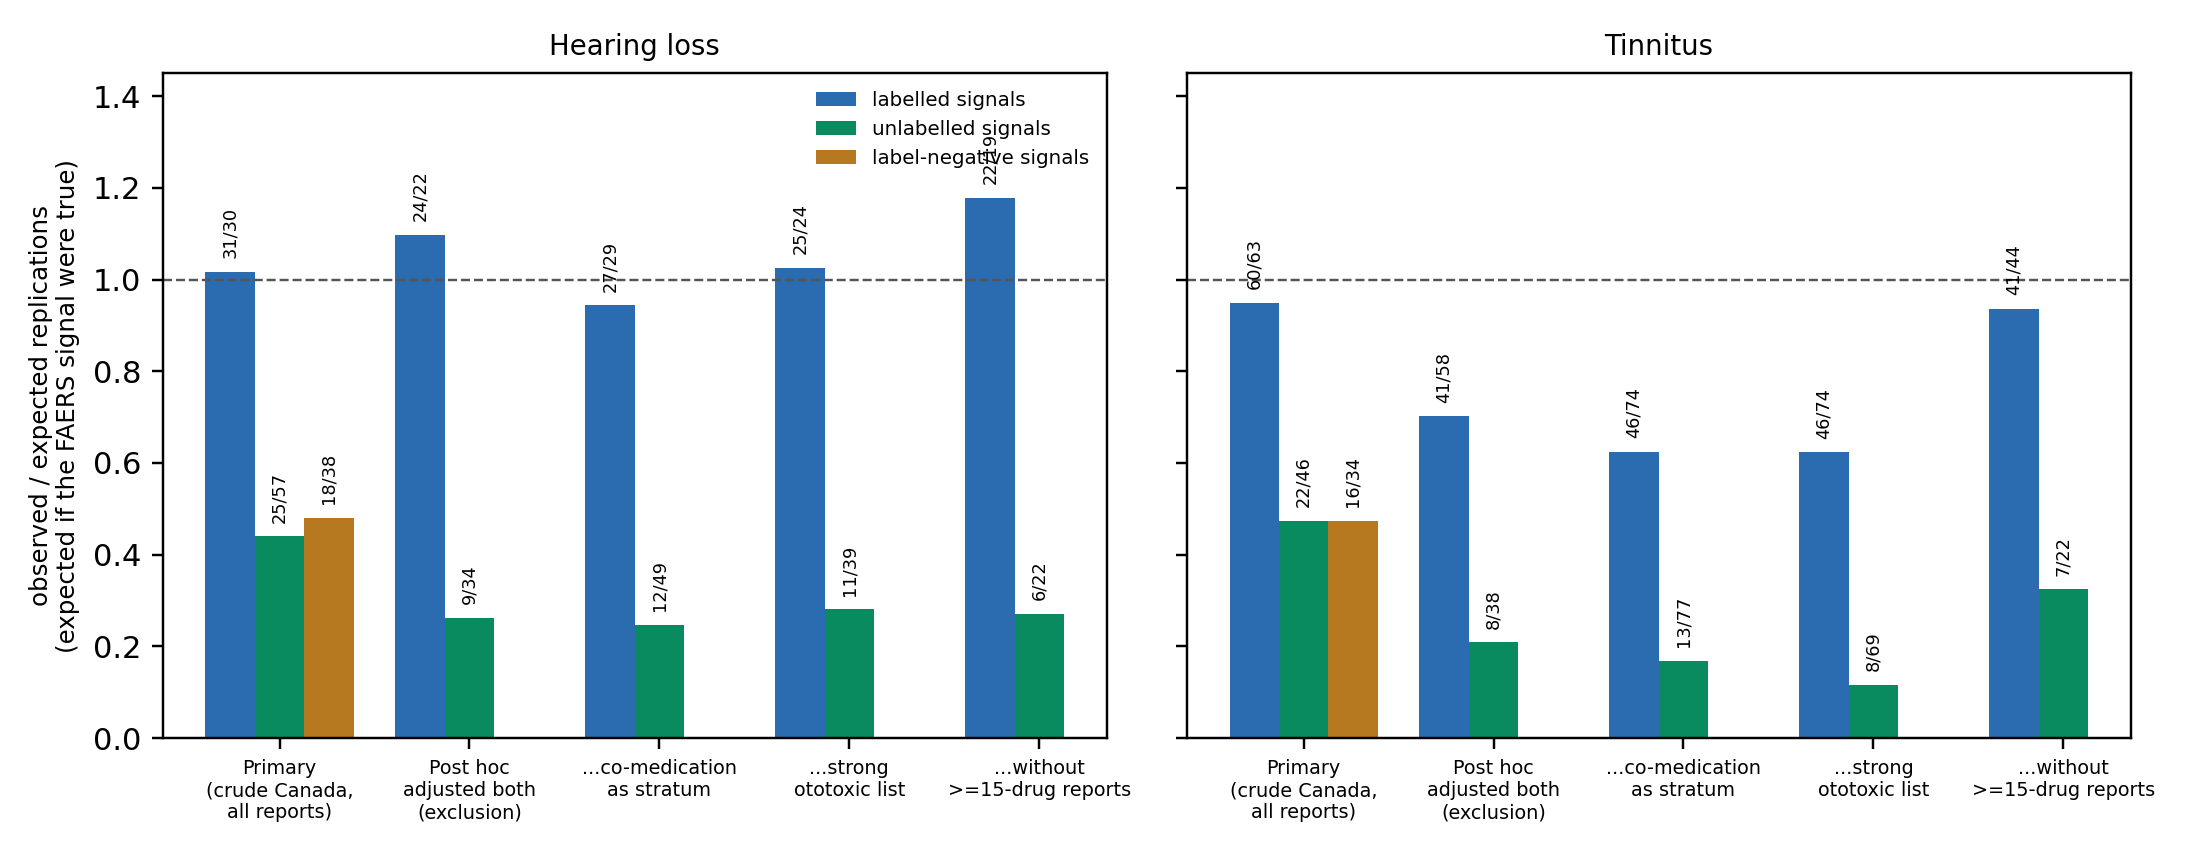
\includegraphics[width=\textwidth]{../figures/replication.png}
\caption{Power-calibrated replication in Canada Vigilance: observed replications divided by those expected if each FAERS
adjusted estimate were true (labels give observed/expected counts). Primary: pre-specified signals, Canada crude estimates,
all reports. Post hoc: both databases adjusted, Canada without solicited reports, four ways of handling co-medication.
A ratio near 1 means signals replicate as their FAERS strength predicts.}
\label{fig:repl}
\end{figure}

\begin{figure}[t]
\centering
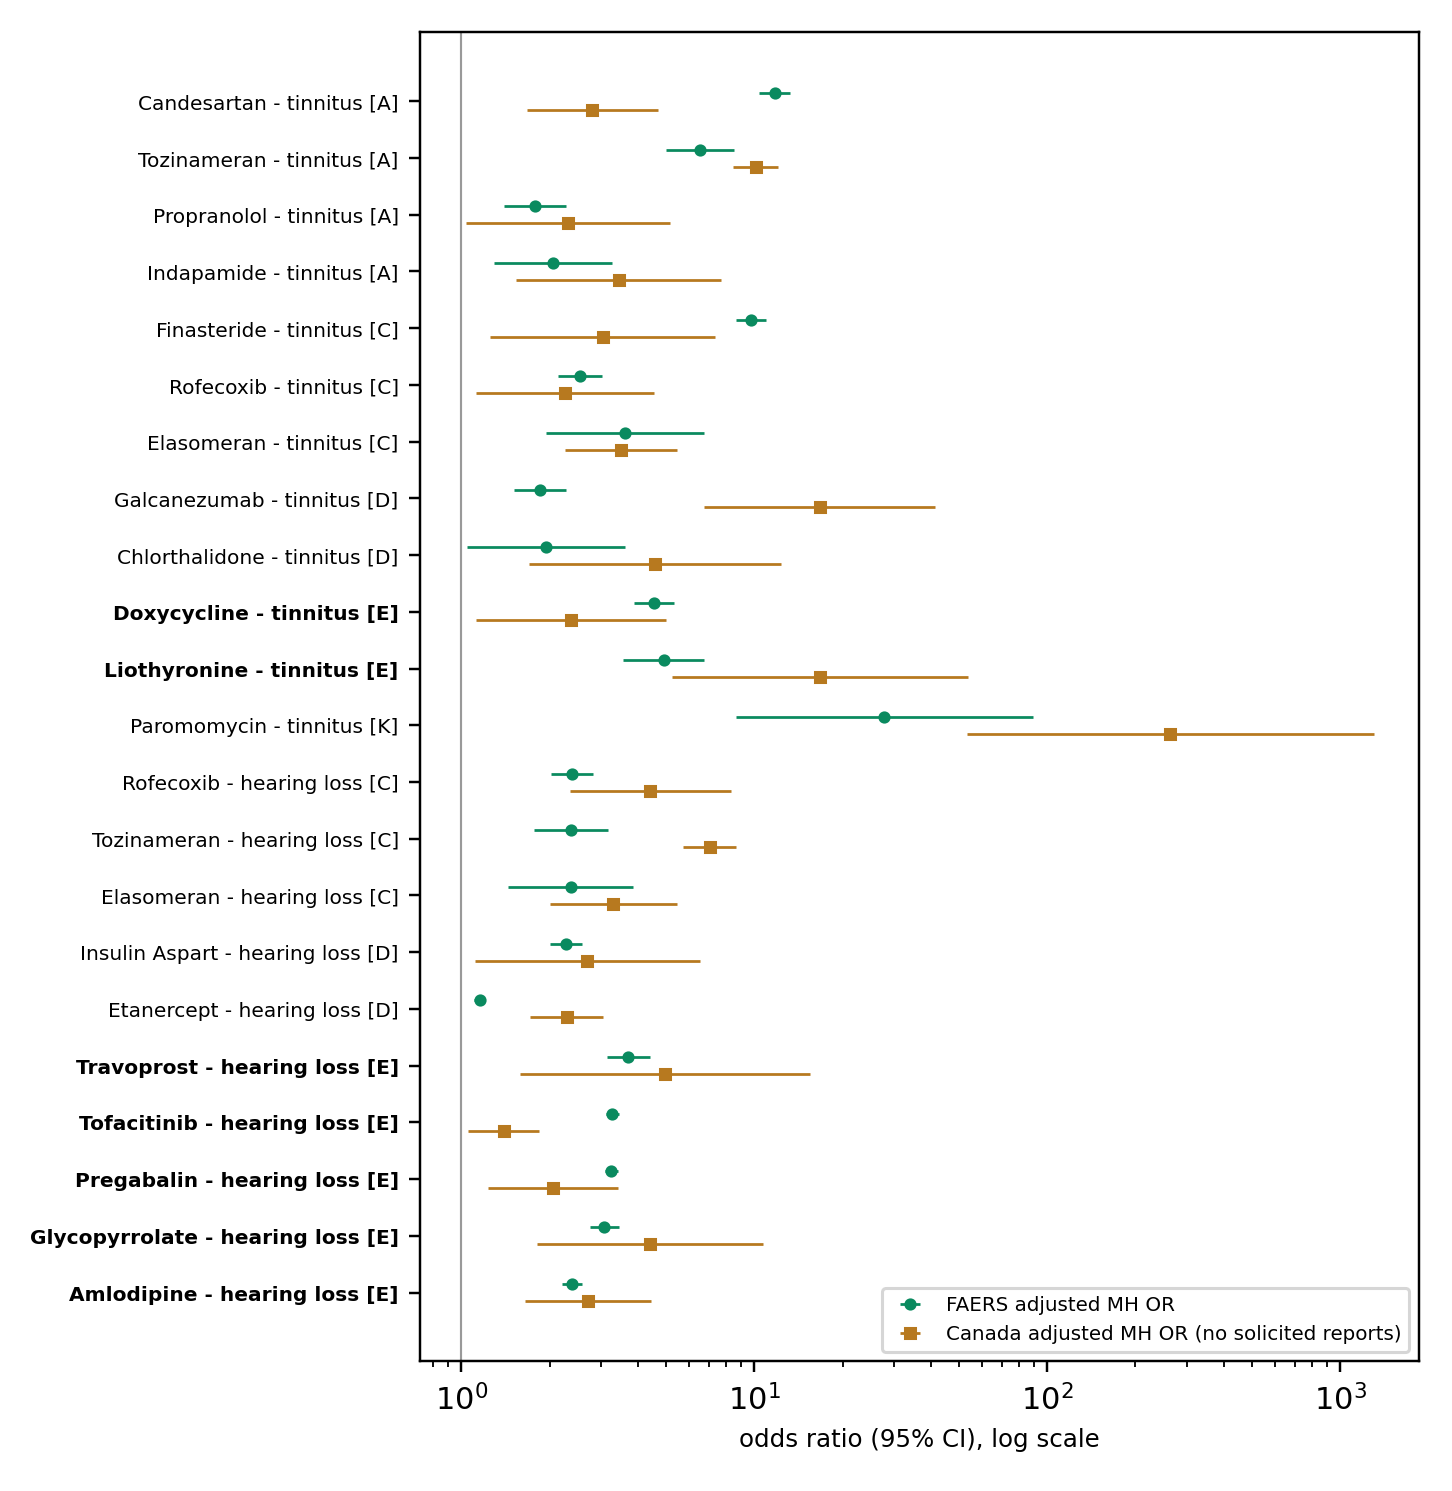
\includegraphics[width=0.85\textwidth]{../figures/candidates.png}
\caption{Robust signals absent from all US labels: FAERS and Canada Vigilance adjusted estimates, with case-review category
(A report cluster; C stimulated reporting; D indication; K established class; E none, bold).}
\label{fig:cand}
\end{figure}


\section{Discussion}
Three findings matter for anyone screening spontaneous reports for ototoxicity. First, adjusting for indication, ototoxic
co-medication, lawyer reports and demographics changed a substantial part of the hearing-loss signal list
(63 of 300 crude signals lost, 73 gained) but did not
improve agreement with labels. Second, replication in an independent national database behaved as a validation test should
for labelled associations---they replicated as often as their strength predicted---but unlabelled signals replicated less
than half as often as predicted, about as often as signals for drugs whose labels are silent on hearing. Third, replication is
not a clean validator on its own: solicited patient-support-programme reports produced ``replications'' for drugs with no
known association, and co-medication bias replicated whenever crude estimates were compared. After adjusted replication and
a review of report provenance, 4 of 22 robust unlabelled signals remained.

These results qualify the previous all-drug screens \cite{li2024,wu2025,liu2025} rather than contradict them. Their
labelled signals largely held; their unlabelled signals mostly did not, and several of the strongest are consistent with how
reports were collected rather than with pharmacology. Tafamidis and sacubitril/valsartan are examples: thousands of consumer
reports in FAERS, consistent with manufacturer programmes in the United States, and none in Canada. The same mechanism
produced spurious Canadian ``replications'' for biologics. Solicited reports are known to distort disproportionality
\cite{psp_solicited}, and their share differs between databases, so report provenance can manufacture both a signal and
its replication. Bias that is shared between databases---co-prescription in standard regimens---also replicates; etoposide
is the clearest example here.

Two inexpensive steps addressed most of what we found: comparing \emph{adjusted} estimates in both databases, and
profiling each case series for concentration---solicited or consumer reports, a single country or year, very drug-dense
reports. The power-calibrated comparison is also simple and avoids the outcome-dependent testability of rules based on
observed counts; it could be extended with empirical calibration against negative controls \cite{schuemie2014} or with
regression-based adjustment for co-reported drugs \cite{caster2010}. We suggest that screens for hearing outcomes report
these provenance indicators for every signal, in line with the case-by-case item of READUS-PV \cite{readuspv,readuspv_ee}.

The remaining candidates are hypotheses with plausible alternative explanations. Pregabalin, an $\alpha_2\delta$ ligand,
had 1{,}703 FAERS hearing-loss reports (adjusted OR
3.25 (3.09--3.43))
that replicated in Canada; a case of reversible, dose-related hearing loss has been described \cite{pregabalin_case}, but
diabetes, neuropathy and age confound \cite{diabetes_hearing}, and its labels list tinnitus and hyperacusis. For amlodipine,
whose labels mention tinnitus, a large cohort found a \emph{lower} risk of sensorineural hearing loss with calcium-channel
blockers \cite{ccb_cohort}, which argues against a causal effect. Doxycycline--tinnitus may reflect pulsatile tinnitus from
drug-induced intracranial hypertension, which is labelled \cite{doxy_iih}, or the infections it treats. None of these should
change practice without studies that have exposure data.

\paragraph{Limitations.} Spontaneous reports lack exposure denominators, and disproportionality measures reporting, not risk
or incidence. The label reference set is imperfect: labels are partly informed by spontaneous reports, list rare events
without causal assessment, and route-specific labels (for example topical gentamicin) blur ingredient-level status; we used
it only to compare methods. Excluding reports with an ototoxic co-medication conditions on a variable that reporters may add
after observing the event; stratifying on it instead gave the same conclusions. Indications are often missing, unreported
co-treatment (for example aminoglycosides in mycobacterial disease) remains, and content deduplication cannot catch
near-duplicate series, which the report-cluster indicator only partly addresses. The Canada Vigilance documentation does not
state that the extract is domestic; restricting it to reports sent directly to Health Canada gave similar results
(39/72 (54\%) of adjusted signals replicated, background
12/58 (21\%)). About 8{,}400 ingredients were screened without multiplicity
correction; the replication and calibration analyses, rather than individual $p$-values, carry the conclusions. Several
analyses---the solicited-report exclusion, the extended indication filter, adjusted-to-adjusted and calibrated replication,
the co-medication variants and the case-level review---were added after the primary results were seen, partly in response
to internal review; they are labelled post hoc and the pre-specified results are reported unchanged. The case-level review
used a written rubric applied by the author and by an AI assessor, not by independent clinicians.

\paragraph{Conclusions.} In FAERS, most drug--hearing-loss signals that are not already on a label do not survive adjustment,
adjusted replication in Canada Vigilance and a review of report provenance; disproportionality analysis remains a
hypothesis-generating tool. Replication in a second spontaneous-reporting database is informative only when both estimates
are adjusted and solicited reports are handled explicitly. The few remaining candidates, led by pregabalin, merit study with
exposure-based designs.

\section*{Statements and declarations}
\textbf{Funding:} no funding was received for this study.
\textbf{Competing interests:} %%COI%%
\textbf{Ethics approval:} not applicable; the study used public, de-identified data.
\textbf{Consent to participate and for publication:} not applicable.
\textbf{Data availability:} FAERS and Canada Vigilance data are publicly available from the FDA and Health Canada; result
tables are in the repository below.
\textbf{Code availability:} code, protocol (\texttt{PROTOCOL.md}, with commit history) and results: %%REPO%%.
\textbf{Author contributions:} OT conceived and designed the study, directed and checked the analysis, and wrote and approved
the manuscript.

\bibliographystyle{unsrtnat}
\bibliography{refs}
\end{document}
